\documentclass[12pt]{article} % use larger type; default would be 10pt
\usepackage[czech]{babel}
\usepackage[utf8]{inputenc} % set input encoding (not needed with XeLaTeX)

%%% PAGE DIMENSIONS
\usepackage{geometry} % to change the page dimensions
% \usepackage[left=2cm,right=2cm,top=2cm,bottom=2cm]{geometry}
\geometry{a4paper}
% \geometry{margin=2in} % for example, change the margins to 2 inches all round
% \geometry{landscape} % set up the page for landscape

\usepackage{graphicx} % support the \includegraphics command and options
\usepackage{wrapfig} % support the wrapfigure section

\usepackage{hyperref} % links in \tableofcontents
\hypersetup{
	colorlinks,
	citecolor=black,
	filecolor=black,
	linkcolor=black,
	urlcolor=black
}

% \usepackage[parfill]{parskip} % Activate to begin paragraphs with an empty line rather than an indent

%%% PACKAGES
\usepackage{booktabs} % for much better looking tables
\usepackage{array} % for better arrays (eg matrices) in maths
\usepackage{paralist} % very flexible & customisable lists (eg. enumerate/itemize, etc.)
\usepackage{verbatim} % adds environment for commenting out blocks of text & for better verbatim
\usepackage{subfig} % make it possible to include more than one captioned figure/table in a single float
% These packages are all incorporated in the memoir class to one degree or another...

%%% HEADERS & FOOTERS
\usepackage{fancyhdr} % This should be set AFTER setting up the page geometry
\pagestyle{fancy} % options: empty , plain , fancy
\renewcommand{\headrulewidth}{0pt} % customise the layout...
\lhead{}\chead{}\rhead{}
\lfoot{}\cfoot{\thepage}\rfoot{}

%%% SECTION TITLE APPEARANCE
\usepackage{sectsty}
\allsectionsfont{\sffamily\mdseries\upshape} % (See the fntguide.pdf for font help)
% (This matches ConTeXt defaults)

%%% ToC (table of contents) APPEARANCE
\usepackage[nottoc,notlof,notlot]{tocbibind} % Put the bibliography in the ToC
\usepackage[titles,subfigure]{tocloft} % Alter the style of the Table of Contents
\renewcommand{\cftsecfont}{\rmfamily\mdseries\upshape}
\renewcommand{\cftsecpagefont}{\rmfamily\mdseries\upshape} % No bold!
\newcommand{\bigsize}{\fontsize{35pt}{20pt}\selectfont}

%%% END Article customizations

\begin{document}
\begin{titlepage}
	
\includegraphics[scale=0.7]{logo.jpg}
	\vspace*{\fill}
	\begin{center}
		\textsc{\LARGE \bigsize Hodnocení stavu životního prostředí v okolí bydliště}\\[1cm]
		Martin Zlámal \\[1cm]
		{\small\em \copyright \ Datum poslední revize \today } \\
		\LaTeX
	\end{center}
	\vspace*{\fill}
\end{titlepage}
\tableofcontents
\listoffigures
%\listoftables
\newpage

% \begin{thebibliography}{999}
% 	\bibitem{dtp}{\em Herout, P.:} {\bf Příprava textů počítačem II.} \\ Vydavatelství Západočeské univerzity, Plzeň~1998
% 	\bibitem{cstug}{\em Dokumentace na serveru sdružení CSTUG} \\ \texttt{http://www.cstug.cz/}
% \end{thebibliography}

\section{Zadání}
Zhodnoťte stav životního prostředí v místě Vašeho trvalého bydliště případně jeho okolí, uveďte způsoby jeho znečišťování a největší znečišťovatele, popište způsob využívání přírodních zdrojů a uveďte Váš návrh na opatření, která by v dané lokalitě přispěla ke zlepšení životního prostředí.

\section{Úvod}
V současné době bydlím ve vesnici Brnířov v západních Čechách jejíž historie sahá až do 16. století. V Brnířově je několik menších firem. Vesnice však úzce sousedí s městem Kdyně, kde je několik větších firem a také čistička odpadních vod.

\subsection{Obec Brnířov}
\begin{wrapfigure}{r}{0.4\textwidth}
	\vspace{-20pt}
	\begin{center}
		
\includegraphics[scale=0.8]{brnirov.jpg}
	\end{center}
	\vspace{-10pt}
	\caption{Znak obce Brnířov}
	\vspace{-20pt}
\end{wrapfigure}
Obec Brnířov se může pyšnit založení prvního jednotného zemědělského družstva JZD v Československu. Koncem roku 2012 zde žilo 377 osob s trvalým pobytem a celková výměra pozemků byla 271 hektarů. V obci je jedna sakrální stavba, konkrétně se jedná o kapličku sv. Martina.

\subsection{Hospodářská činnost}
Podle statistických dat z poloviny roku 2012 zde bylo celkem 90 podnikatelskách subjektů.

Podle právní formy zde bylo evidována jedna státní organizace, dvě akciové společnosti a šest obchodních společností. Nejvíce zde však bylo živnostníků, kterých bylo 65.

Podle převažující činnosti je zde nejvíce obchodů, prodejen a opraven motorových vozidel a spotřebního zboží a pohostinství. Nezanedbatelnou mírou hospodářské činnosti se také podepisuje průmysl, stavebnictví ale například také školství a zdravotnictví.

\subsection{Dopady na životní prostředí}
I přes poměrně bohaté spektrum podnikatelských činností v této obci není žádný přímý zdroj znečišťění životního prostředí. Proto se budu dále zabývat okolím této obce, kde lze již významné znečišťovatele nalézt.

\section{Znečišťovatelé v bezprostředním okolí}
\begin{wrapfigure}{r}{0.6\textwidth}
	\vspace{-20pt}
	\begin{center}
		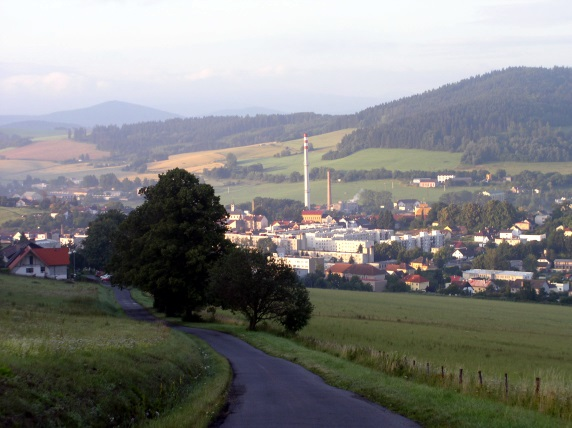
\includegraphics[scale=0.4]{kdyne.jpg}
	\end{center}
	\vspace{-10pt}
	\caption{Kdyni vévodící komín}
	\vspace{-20pt}
\end{wrapfigure}
Obec Brnířov přímo sousedí s městem Kdyně. Toto město bylo významným centrem mnoha manufaktur a dodnes zde sídlí relativně velké fabriky, které se mohou negativně podepisovat na životní prostředí města jako takového, ale i jeho okolí. To je dáno umístěním města v údolí, jemuž dominuje vysoký komín místní teplárny. Ve Kdyni je celá řada významných firem,  které se svým způsobem negativně podepisují na životním prostředí.

\subsection{Významní znečišťovatelé ve Kdyni}
Není možné zde zapsat všechny znečišťovatele, uvadím protopodle mě ty nejvýznamější: 
\begin{description}
	\item[ELITEX Machinery s.r.o.] \hfill \\
	Středně velký podnik strojírenského zaměření. Výroba strojů a linek pro výrobu papírového kartonu a krabic, výroba obráběcích stanic pro dřevozpracující průmysl, výroba extrudovacích strojů, stojanů pro přesné obráběcí stroje, textil a mnohé další.
	\item[APM Automotive s.r.o.] \hfill \\
	Široký sortiment autodílů a autopříslušenství včetně technických kapalin.
	\item[Kdynium a.s.] \hfill \\
	Slévárna vytvářející odlitky metodou voskového vytavitelného modelu. Chemické čistění a obrábění odlitků.
	\item[HAAS Bohemia s.r.o.] \hfill \\
	Drobné díly z polyurethanu a thermoplastu pro automobilový průmysl.
	\item[Teplárny Kdyně] \hfill \\
	Teplárna zajišťující ohřev vody pro většinu Kdyně spalováním uhlí.
	\item[Vodovody a kanalizace města Kdyně s.r.o.]
\end{description}

\section{Znečišťovatelé ve vzdálenějším okolí}
\begin{wrapfigure}{r}{0.4\textwidth}
	\vspace{-20pt}
	\begin{center}
		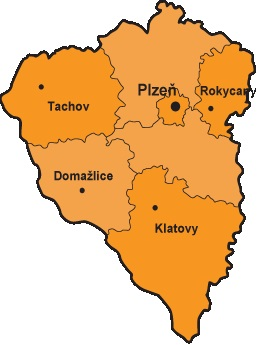
\includegraphics[scale=0.7]{plzensky_kraj.jpg}
	\end{center}
	\vspace{-10pt}
	\caption{Plzeňský kraj}
	\vspace{-20pt}
\end{wrapfigure}
Obec Brnířov i město Kdyně se nacházejí v Plzeňském kraji. Ten leží v západních Čechách. Příroda Plzeňského kraje je velmi rozmanitá a pestrá. Od horských oblastí Šumavy a Českého lesa na západní hranici s Bavorskem přes vrchovinu šumavského podhůří až ke zvlněnému vnitrozemí, všude lze nalézt kulturní krajinu s malebnými městečky a vesnicemi, lesy a vodních ploch. Pro kraj jsou typická hluboko zaříznutá údolí řek: na Šumavě Úhlavy, ve vnitrozemí zejména kaňony Střely u Rabštejna a Berounky pod Plzní.

% http://www.plzensky-kraj.cz/cs/kategorie/zivotni-prostredi

\subsection{Voda}
V kraji se nacházejí dvě oblasti přirozené akumulace vod (Brdy, Šumava) a významnou roli při zásobování obyvatelstva pitnou vodou hrají i vodní nádrže Nýrsko a Lučina. Většinu území kraje odvodňuje Berounka, která vzniká v Plzni soutokem Radbuzy a Mže. Část Klatovska a Sušicko odvodňuje Otava. Obě povodí náleží k úmoří Severního moře. Na území kraje je řada jezer – ledovcová Černé jezero, Čertovo jezero, Prášilské jezero, Laka a hrazené Odlezelské jezero.

\subsection{Odpady}
Největšími zdroji odpadních vod jsou města a obce, menším zdrojem odpadních vod je 
průmysl. Kanalizace pro veřejnou potřebu je vybudována v cca 290 obcích kraje. Část 
této kanalizace, zejména bez koncové ČOV, je provozována samotnými obcemi, zbytek je 
provozován jinými provozovateli. Největšími provozovateli kanalizací pro veřejnou potřebu 
jsou Vodárna Plzeň a.s., JVS a.s. České Budějovice, Vodovody a kanalizace Karlovy Vary 
a.s., Vodovody a kanalizace Starý Plzenec a.s. a další.

Nejvýznamnějšími producenty odpadů v Plzeňském kraji jsou nadále společnosti Plzeňská 
teplárenská a. s., Plzeňská energetika a. s., případně společnosti zabývající se výrobou 
automobilových, především plastových součástek (např. BORGERS CS spol. s r. o. 
Rokycany, Hrádek u Rokycan a Volduchy, EuWe Eugen Wexler ČR, s. r. o. Rokycany, 
IACG s. r. o. Přeštice aj.).

Počet skládek v Plzeňském kraji zůstává zachován. Spíše než uzavírání skládek je snaha 
o jejich další rozšiřování. Hlavními zařízeními k odstraňování odpadů v kraji jsou nadále 
skládky Chotíkov u Plzně, Vysoká u Dobřan, Němčičky u Rokycan, Štěpánovice u Klatov, 
Černošín a Kladruby na Tachovsku a LAZCE-GIS u Horšovského Týna. Na základě žádosti 
společnosti LIDRONE spol. s r. o. bylo ukončeno skládkování nebezpečných odpadů na 
skládce s místním názvem Flóra v Břasích. Konkrétním počinem dalšího rozšiřování kapacity 
skládek bylo vybudování nové kazety na skládce Libkov, kterou provozuje Město Kdyně.

\subsection{Ovzduší}
Největší podíl na emisích amoniaku a VOC v Plzeňském kraji mají malé zdroje (48\% resp. 
61\%), které se významnou měrou podílí rovněž na celkových emisích CO (23\%) a TZL 
(25\%). Velké zdroje produkují nejvíce emisí oxidu siřičitého (82\%). Mobilní zdroje jsou 
největšími producenty emisí tuhých znečišťujících látek (TZL), oxidů dusíku a CO. Na 
celkových emisích se podílejí 49\% u TZL, 66\% u NOx a 69\% u CO.

Mezi nejvýznamnější provozovatele bodových zdrojů emisí v Plzeňském kraji patří: Plzeňská 
teplárenská a.s., Plzeňská energetika a.s., Železárny Hrádek a.s., LASSELSBERGER 
a.s. (Chlumčany a Kaznějov), Klatovská teplárna a.s., Mlékárna Klatovy a.s., Hasit - 
šumavské vápenice a omítkárny a.s. (Velké Hydčice), ŠKODA KOVÁRNY Plzeň s.r.o., 
KDYNIUM a.s., Sklárna Heřmanova Huť a.s., STÖLZLE-UNION a.s. (Heřmanova Huť), 
TRANSTEPLO Kdyně s.r.o., Lear Přeštice.

\subsection{Zemědělství}
Nejlepší podmínky pro zemědělství jsou v Plzeňské kotlině, tam se pěstují převážně obilniny. Plzeňský kraj patří také k významným producentům řepky. Plzeňský kraj má různorodé přírodní podmínky a chov skotu se uskutečňuje zejména v podhorských oblastech, ale díky dobrým vlastnostem travních porostů ve vyšších polohách je lze využít k pasteveckému chovu.V tomto kraji je chováno 161 991 kusů skotu, z toho je 66 386 kusů krav. Tento chov se uskutečňuje zejména v periferních částech kraje.

\subsection{Lesy}
Na území kraje je zastoupeno 9 přírodních lesních oblastí, lesnatost činí 38,8\% a je nad průměrem České republiky, který činí 33,6\%. Z celkové rozlohy připadá přes 80\% na lesy hospodářské, asi 2\% na lesy ochranné a přes 16\% na lesy zvláštního určení. Jde např. o lesy v národním parku, národních přírodních rezervacích, lesy lázeňské nebo lesy v hygienických pásmech ochrany vodních zdrojů. Převažujícími dřevinami jsou smrk a borovice, jejichž monokultury tvoří více než 85\% rozlohy lesů v kraji.

\section{Návrh na opatření ke zlepšení živ. prostředí}
Ačkoliv je v celém regionu značné množsví znečišťovatelů, nemyslím si, že je nutné zavádět nějaká speciální opatření, protože veškeré firmy mají povinost maximálně se starat o to, aby z jejich strany k zásadnímu znečištění životního prostředí nedošlo, jelikož jsou za takový počin nemalé sankce.

\end{document}
